\cotefile{157-3}
\scanpage{18}
\mspage{16}

est l'élément de $\mathrm{Ch}_{\infty}(a,c)$ que voici

\diagram{\begin{tikzcd}[ampersand replacement=\&,column sep=small,row sep=small]
 \& a_{-2} \& a_{-1}\arrow[l]\arrow[r] \& a_0\arrow[d,equal] \& a_1\arrow[l]\arrow[r] \& a_2 \& \cdots \\
 \underset{\mathrm{id}}{\cdots} \& a \& a\arrow[l,"\deleted{\unsure{*}}","\mathrm{id}"']\arrow[r,"0"'] \& \deleted{\unsure{0}}b \& \deleted{\unsure{0}}b\arrow[l,"\unsure{\mathrm{id}}"']\arrow[r,"\text{\textcircled{$\unsure{0|a}$}}"'] \& c \& {}\arrow[l,"\mathrm{id}"'] \& \underset{\mathrm{id}}{\cdots}
\end{tikzcd}}

ce n'est \uline{pas} l'élément nul de $\mathrm{Ch}_{\infty}(a,c)$ !

\deleted{\unsure{Ceci suggère|Cela suggère} de changer la définition de cet élément, de façon à ce que ce soit symétrique par dualité (échange de $+$ et de $-$)
\diagram{\begin{tikzcd}[ampersand replacement=\&,column sep=small,row sep=small]
\cdots \& a_{-2}\arrow[d,equal] \& a_{-1}\arrow[l]\arrow[r]\arrow[d,equal] \& a_0\arrow[d,equal]\arrow[r,shift left=.25ex] \& a_1\arrow[l,shift left=.25ex]\arrow[r]\arrow[d,equal] \& a_2\arrow[d,equal] \& \cdots\\
\underset{\mathrm{id}}{\cdots}\ \cdots \& a \& a\arrow[l,"\mathrm{id}"']\arrow[r] \& 0 \& b\arrow[l]\arrow[r,dash,"\mathrm{id}"'] \& b \& \cdots\ \mathrm{id}\ \cdots
\end{tikzcd}}
\deleted{\unsure{Avec}} cette modification, \deleted{\unsure{les deux flèches}} \inserted{\unsure{on n'a toujours|on a toujours}} pas
\[
 e_{a,b}^{-}\circ e_{b,c}^{+}\overset{?}{=}e_{a,c}
\]}

mais on a des flèches canoniques

\[
 e_{a,b}^{-}\circ e_{b,c}^{+}\ \substack{\longrightarrow\\[-2pt]\longleftarrow}\ e_{a,c}
 \qquad\text{dans }\mathrm{Ch}_{\infty}(a,c)
\]

qui sont l'identité sur tous les sommets sauf celui d'indice $0$. Il y a \unsure{une|un} vérité à développer, comme quoi une paire

\[
 (f:K_\bullet\mathbin{\unsure{-|\longrightarrow}}L_\bullet,\ c)
\]

d'un foncteur entre catégories pointées, et d'un chemin $c$ \deleted{\unsure{de}} $:f(e_{K_\bullet})\longrightarrow e_{L_\bullet}$ définit dans $\mathrm{Hot}_{\bullet}$ une flèche canonique

\[
 \mathrm{hot}_{\bullet}(K_\bullet)\longrightarrow\mathrm{hot}_{\bullet}(L_\bullet)
\]

avec transitivité si on a

\[
 f':L_\bullet\longrightarrow M_\bullet,\quad c':f'(\unsure{e|c}_L)\longrightarrow e_M,
\]
% archive sheet number: 17
\scanpage{19}
\mspage{17}

d'où

\[
 f''=f'\circ f:K_\bullet\longrightarrow M_\bullet,\quad\text{et}\quad c'':f''(e_{K_\bullet})\mathbin{\unsure{-|\longrightarrow}}e_{M_\bullet}
\]

défini ainsi

\diagram{\begin{tikzcd}[ampersand replacement=\&,column sep=small]
\deleted{f'(c):} \& f'(f(e_{\unsure{K|k}}))\arrow[r,"{f'(c)}"]\arrow[rr,bend right=14,"{c''\ \text{par déf.}}"'] \& f'(e_L)\arrow[r,"{c'}"] \& e_M .
\end{tikzcd}}

Cela nous donne donc bel et bien accouplements \unsure{dans} $\mathrm{Hot}_{\bullet}$\inserted{(et aussi \deleted{\unsure{dans}} \inserted{dans} $\unsure{\mathrm{Cat\,hot}_{\bullet}|\mathrm{Cat\,hot}_{:}}$ ?)}. Il est difficile de croire qu'ils pourraient ne pas être associatifs !

\margin{?}

D'ailleurs $\mathrm{Hot}_{\bullet}$, avec le produit cartésien ordinaire$^{*}$, satisfait à l'axiomatique \unsure{de|du} \unsure{tantôt|tantôt prévue} pour $\unsure{\mathcal H|\mathrm H}$, et $\mathrm{Hot}_{\bullet}\longrightarrow\mathrm{Hot}$ est compatible avec ce produit$^{**}$, et avec $\unsure{\Pi|\pi}_0$.

% slanted
\margin{$^{*}$ Non, il faut prendre le produit $X_\bullet\mathbin{\unsure{*|\#}}Y_\bullet$, \deleted{\unsure{$(X\times Y)$}} $(X_\bullet\times Y_\bullet,\ X_\bullet\vee Y_\bullet$ contracté en $e$).}

% slanted
\margin{$^{**}$ Non, mais on \unsure{peut} \unsure{faire} jouer quand-même \unsure{un rôle}}

Si tout ceci marche, on aurait donc une théorie des $\mathrm{Hom\,cat}_{\bullet}$ à valeurs dans $\mathrm{Hot}_{\bullet}$ ; et sans doute aussi pour les $\mathrm{CH}_{\infty}$ comme objets de $\deleted{\unsure{\mathrm{Ind}}}\mathrm{Hot}_{\bullet}$, et non seulement de $\mathrm{Ind\,Hot}_{\unsure{\mathrm{eq}|q}}$.

Mais de \deleted{\unsure{toutes}} façons on ne peut en général laisser tomber $\mathrm{Cat\,hot}$, qui reste importante -- donc il faudrait avoir des objets $\mathrm{CH}_{\infty}(a,b)$ de $\mathrm{Ind\,Cat\,hot}_{\bullet}$, pour avoir une \unsure{côte|cote} bien taillée.

Les $\Pi_0(\unsure{\mathrm{Ch}|\mathcal C}(a,b))$ seront à présent des ensembles pointés, et ce sera pour l'image de l'application nulle $a\xrightarrow{0}b$ \unsure{i.e.} le composé

\[
 a\longrightarrow 0\longrightarrow b
\]
% archive sheet number: 18
\scanpage{20}
\mspage{18}

qu'il faut comparer avec l'élément déduit \unsure{du|des} \unsure{chemin|chemins} \unsure{tronqué|tronqués}

\diagram{\begin{tikzcd}[ampersand replacement=\&,column sep=small,row sep=tiny]
a\arrow[r]\&0\arrow[d,equal]\&b\arrow[l]\&\cdots\\
\&a_0
\end{tikzcd}}

Il faudrait montrer que $0$ est aussi un objet neutre de $M\Sigma^{-1}$, i.e. que

\[
 \deleted{\unsure{\mathrm{Hom}(\,}}\ \unsure{\Pi|\pi}_0(a,0)=\pi_0(0,a)=\{0\}\qquad\text{pour }\deleted{\text{tout}}\ a\in\mathrm{Ob}\,M,
\]

et interpréter \deleted{\unsure{les}} l'élément nul dans $\pi_0(a,b)$ comme l'application nulle dans $M\Sigma^{-1}$. \deleted{\unsure{Il}} En général, il faut des conditions qui assurent (sans que $M$ soit forcément \unsure{ponctuelle|ponctuable}) que

\[
 M\mathbin{\overset{\gamma}{\unsure{-|\longrightarrow}}}M\Sigma^{-1}
\]

commute aux sommes finies, \deleted{\unsure{ou}} aux produits finis (avec $\gamma(\unsure{\phi|\varnothing}_M)=\phi_{M\Sigma^{-1}}$, resp. $\gamma(1_M)=e_{M\Sigma^{-1}}$).

% slanted
\margin{à faire}

Supposons enfin que $M$ soit \uline{additive}, et \deleted{\unsure{soit $k$}} \unsure{même} $k$-linéaire ($k$ un anneau fixé), i.e. on a de plus un hom d'anneaux

\[
 k\longrightarrow\mathrm{End}(\mathrm{id}_M).
\]

On doit supposer quelque compatibilité de $\Sigma$ à la structure additive, p.ex. que la somme directe de deux flèches de $\Sigma$ est dans $\Sigma$, et \deleted{\unsure{de plus}} sans doute qque chose de plus fort, du genre ``lemme des \unsure{cinq}'' pour $\Sigma$. (Mais on ne suppose pas forcément $M$ abélienne donc on aurait du mal à \unsure{formuler|prétendre} un lemme des cinq ?)
% archive sheet number: 19
\scanpage{21}
\mspage{19}

Mais peut-être ici faut-il un axiome plus subtil, p.ex. (si $\Sigma$ \inserted{\unsure{suspension|subséquents}} et $\Omega$ existent$^{*}$) que \deleted{les} \inserted{l'un des} morphismes d'adjonction $\Sigma\Omega\mathbin{\unsure{-|\longrightarrow}}\mathrm{id}$, $\mathrm{id}\longrightarrow\Omega\Sigma$ soit iso, ce qui implique que $\Omega$ resp. $\Sigma$ est pleinement fidèle. \deleted{Dans ce cas, on} En tous cas, l'attente

% slanted
\margin{\unsure{cf|v.} plus bas ce que ça signifie}

naturelle ici, c'est que $\mathrm{Ch}_{\infty}^{\Sigma}(a,b)$ soit non seulement dans $\mathrm{Hot}_{\bullet}$, mais même dans la catégorie \deleted{des complexes \unsure{objets}} \deleted{$\unsure{\mathrm D(k)}$} $\mathrm{D}^{\leq 0}(k\text{-}\mathrm{Mod})$, sous-catégorie pleine de la catégorie dérivée $\mathrm D^{-}(k\text{-}\mathrm{Mod})$ formée des $K$ tels que $H^i(K)=0$ si $i>0$. On peut aussi la noter $\mathrm D_{\geq 0}(k\text{-}\mathrm{Mod})$, l'interprétant en termes de complexes de ``chaînes'' plutôt que de cochaînes. \deleted{\unsure{Dans}}

\uline{Ici} les accouplements doivent correspondre à l'opération $*=\overset{\unsure{\mathbb L|L}}{\otimes}_{k}$ dans $\mathrm D_{\geq 0}(k\text{-}\mathrm{Mod})$, admettant $k$ comme objet unité, et

\[
 \unsure{\Pi|\pi}_0(K_\bullet)=H_0(K_\bullet).
\]

Donc on doit avoir \deleted{\unsure{un produit}}

\[
 \deleted{\unsure{\mathrm{RHom}}}\mathrm{Hom\,cat}_{\deleted{\unsure{\Sigma}}}(a,b)
 \overset{\mathbb L}{\otimes}_k\mathrm{Hom\,cat}(b,c)\longrightarrow\mathrm{Hom\,cat}(a,c),
\]

où cette fois $\mathrm{Hom\,cat}$ désigne l'objet de $\mathrm D_{\geq 0}(k\mathrm{Mod})$, au lieu d'un objet de $\mathrm{Hot}$ seulement, ou de $\mathrm{Hot}_{\bullet}$. \unsure{Alors utiliser|On utilise} les foncteurs

\[
 \mathrm D_{\geq 0}(k\,\mathrm{Mod})\longrightarrow\mathrm{Hot}_{\unsure{\bullet|*}}\longrightarrow\mathrm{Hot}
\]
% archive sheet number: 20
\scanpage{22}
\mspage{20}

\margin{dans $\mathrm{Hot}_{\bullet}$.}

pour faire le lien avec la théorie \unsure{primitive|première|ponctuée}, ou théorie générale \unsure{des|dans} $\mathrm{Hot}_{\bullet}$. Si on désigne par

\[
 \gamma:\mathrm D_{\geq 0}(k)\mathbin{\unsure{-|\longrightarrow}}\mathrm{Hot}_{\bullet}
\]

le premier de ces foncteurs, il ne commute pas aux produits $*$ ($\overset{\unsure{\mathbb L|L}}{\otimes}_k$ et $\times$ \unsure{resp.$^t$}), mais on a, pour $P_\bullet,Q_\bullet$ variables dans $\mathrm D_{\geq}(k)$, une flèche fonctorielle canonique

\[
 \gamma(P_\bullet\overset{\mathbb L}{\otimes}_k Q_\bullet)
 \xleftarrow{\mathrm{can.}}\underset{\text{``$k$-bilinéaire''}}{\gamma(P)\times\gamma(Q)}
\]

Ce qui montre que de donner des accouplements

\[
 P_{\unsure{\bullet}}\mathbin{*}Q\xrightarrow{\unsure{c_k|c_K}}R,
\]

d'où

\[
 \gamma(P\mathbin{\unsure{*|\circ}}Q)\xrightarrow{\gamma(\unsure{c_k|\varphi})}\gamma(R),\tag*{$(*)$}
\]

est l'un et l'autre plus fin que de se donner seulement

\[
 \gamma(P)\mathbin{*}\gamma(Q)\xrightarrow{c_\bullet}\gamma(R)\tag*{$(*')$}
\]

vu que \inserted{une donnée} $(*)$ implique une donnée $(*')$ par

\diagram{\begin{tikzcd}[ampersand replacement=\&,row sep=small]
 \&\gamma(P*Q)\arrow[dr,"{\gamma(c)}"]\&\\
 \gamma(P)\times\gamma(Q)\arrow[ur,"\mathrm{can.}"]\arrow[rr,"{c_\bullet}"']\&\&\gamma(R).
\end{tikzcd}}

Ceci vu, on s'attend bien à avoir une théorie \uline{forte} des accouplements
% archive sheet number: 21
\scanpage{23}
\mspage{21}

\[
 \mathrm{Hom\,cat}_k(a,b)\overset{\unsure{\mathbb L|L}}{\otimes}_k\mathrm{Hom\,cat}_k(b,c)\mathbin{\unsure{-|\longrightarrow}}\mathrm{Hom\,cat}_k(a,c),
\]

d'où on déduira des accouplements plus faibles dans $\mathrm{Hot}_{\bullet}$ (au lieu de $\mathrm D_{\geq 0}(k)$)

\[
 \mathrm{Hom\,cat}_{\mathrm{Hot}_{\bullet}}(a,b)\times
 \mathrm{Hom\,cat}_{\mathrm{Hot}_{\bullet}}(b,c)\longrightarrow
 \mathrm{Hom\,cat}_{\mathrm{Hot}_{\bullet}}(a,c).
\]

$3^\circ)$ Revenant au cas $M$ ponctuée sans plus, Quillen définit, pour $a,b$ dans $M$

\[
 \unsure{\Pi|\pi}_{\unsure{1}}(a,b)=\Pi_1(a,b;0_a,0_b)
\]

\margin{comme bifoncteur sur $(M\Sigma^{-1})^{\unsure{\circ|0}}\times M\Sigma^{-1}$}

(avec les notations du $1^\circ)$). Si ce que j'avance sans preuves dans $1^\circ)$ est vrai, il doit s'ensuivre qu'on a un isom. can.

\[
 \Pi_1(a,b)\simeq\Pi_{\unsure{1|2}}\bigl(\mathrm{Ch}^{\Sigma}_{\infty}(a,b)\bigr)
\]

où $\mathrm{Ch}^{\Sigma}_{\infty}(a,b)$ est vu comme objet de $\mathrm{Hot}_{\bullet}$, donc son $\Pi_1$ est défini\unsure{.|:} On a \deleted{\unsure{ainsi}} \inserted{en tous cas} sans aucune référence à des cofibrations et des fibrations, un bifoncteur à valeurs dans Groupes, composé \deleted{des}

\diagram{\begin{tikzcd}[ampersand replacement=\&,column sep=large]
(M\Sigma^{-1})^{\circ}\times M\Sigma^{-1}
\arrow[r,"{(a,b)\mapsto\mathrm{Ch}^{\Sigma}_{\infty}(a,b)}"]\&
\mathrm{Hot}_{\bullet}\arrow[r,dash,"\Pi_1"]\&(\mathrm{Groupes})
\end{tikzcd}}

Si pour $a$ fixé, $b$ variable, \deleted{$\Pi_1(a,b)$}

\[
 b\mathbin{\unsure{-|\mapsto}}\Pi_1(a,b)
\]

est représentable, on note l'objet qui le représente par $\Sigma(a)$ \deleted{\unsure{$f$}} (\uline{suspension} -- ne pas confondre ce $\Sigma$ avec $\Sigma\subset\mathrm{Fl}(M)$, qu'il vaut mieux maintenant noter $W$, comme ``weak \unsure{equivalence|equivalences}''). Donc
% archive sheet number: 22
\scanpage{24}
\mspage{22}

\[
 \mathrm{Hom}(\Sigma a,b)\simeq\unsure{\Pi|\pi}_1(a,b),
\]

et $\Sigma a$ dépend fonctoriellement de $a$, sous réserve d'existence. S'il existe tjrs, on a

\[
 \Sigma:MW^{-1}\mathbin{\unsure{-|\longrightarrow}}MW^{-1}.
\]

On définit de \unsure{$\overline{\rm m}$|$=$|même}, sous réserve d'existence,

\[
 \Omega:MW^{-1}\mathbin{-}MW^{-1}
\]

par

\[
 \mathrm{Hom}(a,\Omega b)\simeq\Pi_1(a,b),
\]

et si tous les deux existent, on a la formule d'adjonction

\[
 \mathrm{Hom}(\Sigma a,b)\simeq\mathrm{Hom}(a,\Omega b)
 \quad(\simeq\Pi_1\mathrm{Hom\,cat}_{\mathrm{Hot}_{\bullet}}(a,b)).
\]

\deleted{\unsure{Attente}} L'existence de
\[
 \begin{aligned}
 \Omega:MW^{-1}\longrightarrow MW^{-1},&\ \text{ou de}\\
 \Sigma:MW^{-1}\mathbin{-}MW^{-1},&
 \end{aligned}
\]
voire même des deux à la fois, apparaît comme une hypothèse$^{\text{\textcircled{\scriptsize a}}}$ extrêmement forte sur $(M,W)$, \deleted{c'est} Cette \deleted{hypothèse} \inserted{\unsure{condition}} \uline{plus} celle$^{\text{\textcircled{\scriptsize b}}}$ que les $\underline{\mathrm{Ch}}_{\infty}(a,b)$ soient \inserted{\unsure{homotopiq$^{\rm mt}$|homotopiquement}} des Cat. de

\unsure{Th.-Kan|Th.-kan}, \deleted{\unsure{ou que}} ou (ce qui revient au même, à peu de choses près ?) que $Y\longmapsto\mathrm{Hom}_{M(Y)W_Y^{-1}}(a_Y,b_Y)$ transforme Hot-équivalences de Cat en bijections (ne serait-ce que pour $Y$ fini $\ldots$), semble le \unsure{test} crucial pour savoir si ``$M,\Sigma$ se prête à une théorie \deleted{de} \deleted{\unsure{$\Sigma$}} homotopique ``dans $M$''''. Je doute \unsure{que}\deleted{\unsure{ce}}
% archive sheet number: 23
\scanpage{25}
\mspage{23}

ces \deleted{\unsure{hypothèses}} conditions puissent être satisfaites pour $M$ finie, sauf dans le cas trivial où \inserted{$M=\varnothing$, ou} $M\Sigma^{-1}$ est équivalente à la catégorie ponctuelle.

Un troisième test \textcircled{\scriptsize c} qui me paraît important (mais peut-être ça résulte du reste ?), c'est les formules dans $\mathrm{Hot}_{\bullet}$

\[
 \left\{\begin{aligned}
 \mathrm{Hom\,cat}_{\bullet}(\Sigma a,b)&\simeq\mathrm{Hom\,cat}_{\bullet}(a,\Omega b)\\
 &\simeq\Omega\,\mathrm{Hom\,cat}_{\bullet}(a,b),
 \end{aligned}\right.\tag*{$(*)$}
\]

où \unsure{le|les} $\mathrm{Hom\,cat}_{\bullet}$ \unsure{désigne|désignent} \unsure{le|les} $\mathrm{Hom}$ \unsure{externes|externe} à valeurs dans $\mathrm{Hot}_{\bullet}$. Il faut les voir séparément (sous conditions d'existence soit de $\Omega$, soit de $\Sigma$) comme deux formules ``duales'' l'une de l'autre

\[
 \left\{\begin{aligned}
 \mathrm{Hom\,cat}_{\bullet}(a,\Omega b)&\simeq\Omega\,\mathrm{Hom\,cat}_{\bullet}(a,b)\\
 \mathrm{Hom\,cat}_{\bullet}(\Sigma a,b)&\simeq\Omega\,\mathrm{Hom\,cat}_{\bullet}(a,b),
 \end{aligned}\right.\tag*{$(**)$}
\]

isomorphismes de \uline{groupes} dans $\mathrm{Hot}_{\bullet}$ (\uline{NB} $\Omega b$ est un objet groupe de $M\underline W^{-1}$, car il représente un foncteur à valeurs dans $\mathrm{Gr}$, et de même $\Sigma a$ est un cogroupe de $MW^{-1}$. Le foncteur $\mathrm{Hom\,cat}_{\bullet}(a,\deleted{\unsure{y}}\,\unsure{y})$ \deleted{\unsure{transforme}} \inserted{doit} commuter aux produits finis, et donc transformer \inserted{objets} groupes en \unsure{itous|itou}.

% slanted
\margin{le foncteur $\Omega$ doit provenir d'un endom. du \uline{dérivateur} $\unsure{\mathbb D|\mathrm D}=\mathbb D_{M,W}$, et celui-\deleted{\unsure{ci}}ci doit être exact à gauche, et dualement pour $\Sigma$}

Et de même \deleted{\unsure{$y$}} $x\mathbin{\unsure{\mapsto|-}}\mathrm{Hom\,cat}_{\bullet}(\unsure{a|x},b)$ doit transformer sommes finies en produits finis, donc cogroupes en groupes.)

Je \unsure{me|ne} suis convaincu que les \unsure{isom$^t$|isom.} $(**)$ n'ont de chances d'exister que si on a la condition préalable \textcircled{\scriptsize b}.
% archive sheet number: 24
\scanpage{26}
\mspage{24}

3. \uline{Essai de construction du foncteur} $\Omega$

Il n'y a sans doute guère de chances de prouver quelque chose sur le foncteur

\[
 \Omega:MW^{-1}\longrightarrow MW^{-1},
\]

sans \unsure{fournir|donner} au moins une \uline{construction} plus ou moins explicite de celui-ci. Je vais essayer, \deleted{\unsure{en}} en m'inspirant de Quillen, de dégager des conditions générales sur $M,W$ (plus générales que celles de Quillen) qui assurent l'existence de $\Omega$, et permettent de le construire. L'idée géométrique remonte à Serre-Cartan. \deleted{c'est} Il s'agit, pour un objet $a$ de $M$, de construire un objet \deleted{\unsure{pour}} $\mathrm{Ch}(\deleted{\unsure{a}}S)$ \uline{dans $M$}, jouant le rôle d'un \deleted{\unsure{tel}} ``espace de chemins'', et qui doit \deleted{\unsure{satisfaire à la condition}} \inserted{\unsure{s'inclure|s'insérer} dans un diagramme de} factorisation de \deleted{\unsure{\(\Delta\)}} $\mathrm{diag}_S:S\longrightarrow S\times S$ (on suppose que dans $M$ les \deleted{produits} \inserted{\unsure{lims|lims.}} finies, \inserted{donc les produits finis,} existent)

\diagram{\begin{tikzcd}[ampersand replacement=\&,row sep=small,column sep=small]
 S\arrow[d,"i_S"]\arrow[dd,bend right=22,"{\mathrm{diag}_S}"']\&\\
 \mathrm{Ch}(S)\arrow[d,"{\unsure{p|P}_S}"]\&\\
 S\times S\&e\arrow[l]
\end{tikzcd}}

La propriété essentielle, c'est que $p$ soit une ``\uline{fibration}'' (dans un sens convenable, à dégager).
% archive sheet number: 25
\scanpage{27}
\mspage{25}

A titre accessoire il peut être utile (peut-être) que $i$ soit une ``cofibration''$^{+}$. On définit $\Omega(S)$ comme la fibre de $\mathrm{Ch}(S)$ sur $S\times S$ (par rapport à l'unique morphisme $e=e_M\mathbin{\unsure{-|\longrightarrow}}S\times S$, où $e_M$ est l'objet \deleted{\unsure{neutre}} \inserted{nul} de $M$).

% slanted
\margin{et peut-être que $S\longrightarrow e$ \unsure{soit|doit} également une ``fibration'' ?}

\diagram{\begin{tikzcd}[ampersand replacement=\&,row sep=small]
 \mathrm{Ch}(S)\arrow[d]\&\Omega S\arrow[l]\arrow[d]\\
 S\times S\&e\arrow[l]\quad .
\end{tikzcd}}

C'est un objet de $M$, qu'on regardera surtout comme un objet de $MW^{-1}$. Il faut s'assurer qu'on a une \deleted{\unsure{isom.}} \inserted{bij.} fonctorielle en $T$ dans $MW^{-1}$ :

\diagram{\begin{tikzcd}[ampersand replacement=\&,row sep=small,column sep=tiny]
 \unsure{\Pi|\pi}_1\underline{\mathrm{Ch}}_{\infty}^{W}(T,S)\arrow[d,equal,"\text{déf}"]\&[-5pt]\simeq\&
 \mathrm{Hom}_{MW^{-1}}(T,\Omega S)\arrow[d,equal,"\text{déf}"]\\
 \Pi_1(T,S)\&\&\Pi_0(\underline{\mathrm{Ch}}^{W}_{\infty}(T,\Omega S)).
\end{tikzcd}}

Pour cela il s'impose de comparer

\diagram{\begin{tikzcd}[ampersand replacement=\&,row sep=large,column sep=tiny]
 \underline{\mathrm{Ch}}^{W}_{\infty}(T,\Omega S)\&\text{et}\&
 \Omega_{\mathrm{Hot}_{\bullet}}\bigl(\underline{\mathrm{Ch}}^{W}_{\infty}(T,S)\bigr)
 \arrow[d,equal,"{\substack{\text{``par ``définition''}\\\text{pour }\Omega\text{ de }\mathrm{Hot}_{\bullet}}}"]\\
 \&\&\underline{\mathrm{Ch}}_{\infty}\bigl(\underline{\mathrm{ch}}^{W}_{\infty}(T,S);\unsure{\sigma|0|o},\sigma\bigr),
\end{tikzcd}}

puisqu'il s'agit \deleted{\unsure{de}} \unsure{d'y|de} construire une bijection entre leurs $\Pi_0$.
% archive sheet number: 26
\scanpage{28}
\mspage{\handwritten{4}}

\deleted{En fonction des remarques que vous me ferez, je modifierai ce dossier soit en le complétant, soit en l'allégeant (car il y a sûrement des choses inutiles). Il faut qu'il serve à ceux qui vont se battre et à ceux qui vont les aider. Son objectif essentiel est de convaincre qu'il est possible de s'organiser avec les moyens du bord. Quand j'ai \unsure{démarre|démarré} dans cette affaire je n'avais rien, aujourd'hui les documents forment une pile d'un mètre d'épaisseur. En continuant notre collaboration nous finirons par faire un outil utile à tous.}

\deleted{Au plaisir de vous lire}\\

\deleted{\handwritten{\uline{\unsure{IC\uline{L}|JC\uline{L}|LC\uline{L}}}}}\\

\deleted{à La Ribe le 7 novembre I986}\\
% archive sheet number: 27
\scanpage{29}

Comparaison de $\mathrm{Cat}$ avec $\unsure{\Delta^{\wedge}|\widehat{\Delta}|\Delta^{1}}$

X
% archive sheet number: 28
\scanpage{30}

% printed form
\texttt{//*\quad PREDONTA1156\qquad I}

\figure{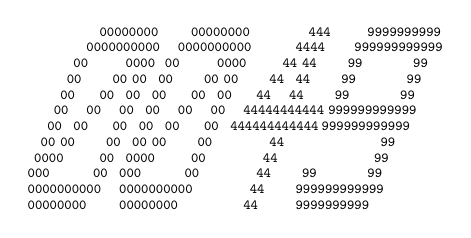
\begin{tikzpicture}[x=.083cm,y=-.20cm,every node/.style={anchor=base west,inner sep=0pt,font=\fontsize{4.5}{5}\selectfont\ttfamily}]
\node at (11,0) {00000000}; \node at (25,0) {00000000}; \node at (43,0) {444}; \node at (52,0) {9999999999};
\node at (9,1) {0000000000}; \node at (23,1) {0000000000}; \node at (41,1) {4444}; \node at (50,1) {999999999999};
\node at (7,2) {00}; \node at (15,2) {0000}; \node at (21,2) {00}; \node at (29,2) {0000}; \node at (39,2) {44}; \node at (42,2) {44}; \node at (49,2) {99}; \node at (59,2) {99};
\node at (6,3) {00}; \node at (13,3) {00}; \node at (16,3) {00}; \node at (20,3) {00}; \node at (27,3) {00}; \node at (30,3) {00}; \node at (37,3) {44}; \node at (41,3) {44}; \node at (48,3) {99}; \node at (58,3) {99};
\node at (5,4) {00}; \node at (11,4) {00}; \node at (15,4) {00}; \node at (19,4) {00}; \node at (25,4) {00}; \node at (29,4) {00}; \node at (35,4) {44}; \node at (40,4) {44}; \node at (47,4) {99}; \node at (57,4) {99};
\node at (4,5) {00}; \node at (9,5) {00}; \node at (14,5) {00}; \node at (18,5) {00}; \node at (23,5) {00}; \node at (28,5) {00}; \node at (33,5) {44444444444}; \node at (46,5) {999999999999};
\node at (3,6) {00}; \node at (7,6) {00}; \node at (13,6) {00}; \node at (17,6) {00}; \node at (21,6) {00}; \node at (27,6) {00}; \node at (31,6) {444444444444}; \node at (45,6) {999999999999};
\node at (2,7) {00}; \node at (5,7) {00}; \node at (12,7) {00}; \node at (16,7) {00}; \node at (19,7) {00}; \node at (26,7) {00}; \node at (37,7) {44}; \node at (54,7) {99};
\node at (1,8) {0000}; \node at (11,8) {00}; \node at (15,8) {0000}; \node at (25,8) {00}; \node at (36,8) {44}; \node at (53,8) {99};
\node at (0,9) {000}; \node at (10,9) {00}; \node at (14,9) {000}; \node at (24,9) {00}; \node at (35,9) {44}; \node at (42,9) {99}; \node at (52,9) {99};
\node at (0,10) {0000000000}; \node at (14,10) {0000000000}; \node at (34,10) {44}; \node at (41,10) {999999999999};
\node at (0,11) {00000000}; \node at (14,11) {00000000}; \node at (33,11) {44}; \node at (41,11) {9999999999};
\end{tikzpicture}}

\figure{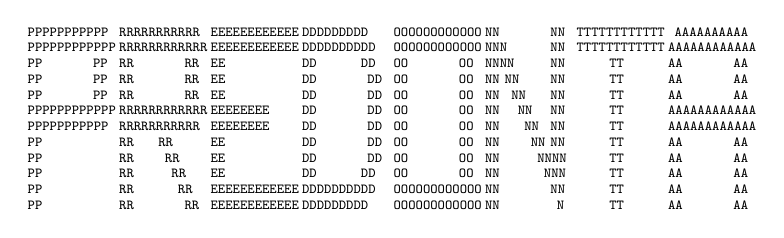
\begin{tikzpicture}[x=.083cm,y=-.20cm,every node/.style={anchor=base west,inner sep=0pt,font=\fontsize{4.5}{5}\selectfont\ttfamily}]
\node at (0,0) {PPPPPPPPPPP}; \node at (14,0) {RRRRRRRRRRR}; \node at (28,0) {EEEEEEEEEEEE}; \node at (42,0) {DDDDDDDDD}; \node at (56,0) {OOOOOOOOOOOO}; \node at (70,0) {NN}; \node at (80,0) {NN}; \node at (84,0) {TTTTTTTTTTTT}; \node at (99,0) {AAAAAAAAAA};
\node at (0,1) {PPPPPPPPPPPP}; \node at (14,1) {RRRRRRRRRRRR}; \node at (28,1) {EEEEEEEEEEEE}; \node at (42,1) {DDDDDDDDDD}; \node at (56,1) {OOOOOOOOOOOO}; \node at (70,1) {NNN}; \node at (80,1) {NN}; \node at (84,1) {TTTTTTTTTTTT}; \node at (98,1) {AAAAAAAAAAAA};
\node at (0,2) {PP}; \node at (10,2) {PP}; \node at (14,2) {RR}; \node at (24,2) {RR}; \node at (28,2) {EE}; \node at (42,2) {DD}; \node at (51,2) {DD}; \node at (56,2) {OO}; \node at (66,2) {OO}; \node at (70,2) {NNNN}; \node at (80,2) {NN}; \node at (89,2) {TT}; \node at (98,2) {AA}; \node at (108,2) {AA};
\node at (0,3) {PP}; \node at (10,3) {PP}; \node at (14,3) {RR}; \node at (24,3) {RR}; \node at (28,3) {EE}; \node at (42,3) {DD}; \node at (52,3) {DD}; \node at (56,3) {OO}; \node at (66,3) {OO}; \node at (70,3) {NN}; \node at (73,3) {NN}; \node at (80,3) {NN}; \node at (89,3) {TT}; \node at (98,3) {AA}; \node at (108,3) {AA};
\node at (0,4) {PP}; \node at (10,4) {PP}; \node at (14,4) {RR}; \node at (24,4) {RR}; \node at (28,4) {EE}; \node at (42,4) {DD}; \node at (52,4) {DD}; \node at (56,4) {OO}; \node at (66,4) {OO}; \node at (70,4) {NN}; \node at (74,4) {NN}; \node at (80,4) {NN}; \node at (89,4) {TT}; \node at (98,4) {AA}; \node at (108,4) {AA};
\node at (0,5) {PPPPPPPPPPPP}; \node at (14,5) {RRRRRRRRRRRR}; \node at (28,5) {EEEEEEEE}; \node at (42,5) {DD}; \node at (52,5) {DD}; \node at (56,5) {OO}; \node at (66,5) {OO}; \node at (70,5) {NN}; \node at (75,5) {NN}; \node at (80,5) {NN}; \node at (89,5) {TT}; \node at (98,5) {AAAAAAAAAAAA};
\node at (0,6) {PPPPPPPPPPP}; \node at (14,6) {RRRRRRRRRRR}; \node at (28,6) {EEEEEEEE}; \node at (42,6) {DD}; \node at (52,6) {DD}; \node at (56,6) {OO}; \node at (66,6) {OO}; \node at (70,6) {NN}; \node at (76,6) {NN}; \node at (80,6) {NN}; \node at (89,6) {TT}; \node at (98,6) {AAAAAAAAAAAA};
\node at (0,7) {PP}; \node at (14,7) {RR}; \node at (20,7) {RR}; \node at (28,7) {EE}; \node at (42,7) {DD}; \node at (52,7) {DD}; \node at (56,7) {OO}; \node at (66,7) {OO}; \node at (70,7) {NN}; \node at (77,7) {NN}; \node at (80,7) {NN}; \node at (89,7) {TT}; \node at (98,7) {AA}; \node at (108,7) {AA};
\node at (0,8) {PP}; \node at (14,8) {RR}; \node at (21,8) {RR}; \node at (28,8) {EE}; \node at (42,8) {DD}; \node at (52,8) {DD}; \node at (56,8) {OO}; \node at (66,8) {OO}; \node at (70,8) {NN}; \node at (78,8) {NNNN}; \node at (89,8) {TT}; \node at (98,8) {AA}; \node at (108,8) {AA};
\node at (0,9) {PP}; \node at (14,9) {RR}; \node at (22,9) {RR}; \node at (28,9) {EE}; \node at (42,9) {DD}; \node at (51,9) {DD}; \node at (56,9) {OO}; \node at (66,9) {OO}; \node at (70,9) {NN}; \node at (79,9) {NNN}; \node at (89,9) {TT}; \node at (98,9) {AA}; \node at (108,9) {AA};
\node at (0,10) {PP}; \node at (14,10) {RR}; \node at (23,10) {RR}; \node at (28,10) {EEEEEEEEEEEE}; \node at (42,10) {DDDDDDDDDD}; \node at (56,10) {OOOOOOOOOOOO}; \node at (70,10) {NN}; \node at (80,10) {NN}; \node at (89,10) {TT}; \node at (98,10) {AA}; \node at (108,10) {AA};
\node at (0,11) {PP}; \node at (14,11) {RR}; \node at (24,11) {RR}; \node at (28,11) {EEEEEEEEEEEE}; \node at (42,11) {DDDDDDDDD}; \node at (56,11) {OOOOOOOOOOOO}; \node at (70,11) {NN}; \node at (81,11) {N}; \node at (89,11) {TT}; \node at (98,11) {AA}; \node at (108,11) {AA};
\end{tikzpicture}}

{\fontsize{4.4}{5.5}\selectfont\ttfamily ****A\ \ START\ \ JOB 1156\ \ PREDONTA\hfill ROOM\hfill 4.10.32 PM 15 NOV 82\ \ R6.PR1\ \ \ SYS JES2\ \ JOB 1156\ \ START\ \ A****}

{\fontsize{4.4}{5.5}\selectfont\ttfamily ****A\ \ START\ \ JOB 1156\ \ PREDONTA\hfill ROOM\hfill 4.10.32 PM 15 NOV 82\ \ R6.PR1\ \ \ SYS JES2\ \ JOB 1156\ \ START\ \ A****}

{\fontsize{4.4}{5.5}\selectfont\ttfamily ****A\ \ START\ \ JOB 1156\ \ PREDONTA\hfill ROOM\hfill 4.10.32 PM 15 NOV 82\ \ R6.PR1\ \ \ SYS JES2\ \ JOB 1156\ \ START\ \ A****}

{\fontsize{4.4}{5.5}\selectfont\ttfamily ****A\ \ START\ \ JOB 1156\ \ PREDONTA\hfill ROOM\hfill 4.10.32 PM 15 NOV 82\ \ R6.PR1\ \ \ SYS JES2\ \ JOB 1156\ \ START\ \ A****}

{\fontsize{4.4}{5.5}\selectfont\ttfamily ****A\ \ START\ \ JOB 1156\ \ PREDONTA\hfill ROOM\hfill 4.10.32 PM 15 NOV 82\ \ R6.PR1\ \ \ SYS JES2\ \ JOB 1156\ \ START\ \ A****}

{\fontsize{4.4}{5.5}\selectfont\ttfamily ****A\ \ START\ \ JOB 1156\ \ PREDONTA\hfill ROOM\hfill 4.10.32 PM 15 NOV 82\ \ R6.PR1\ \ \ SYS JES2\ \ JOB 1156\ \ START\ \ A****}

\texttt{- DERNIERE MISE A JOUR DE JOURNAL : 10-11-82}

\texttt{- DEMONSTRATION DU MATERIEL CORAIL (SEMS) LE JEUDI 25/11/82 AU CNUSC DE 8 H A 18 HEURES .}

\texttt{-{}-{}-{}-{}-{}-{}-> ATTENTION !!!}

\texttt{LE MERCREDI 17 NOVEMBRE MISE EN EXPLOITATION DE LA NOUVELLE VERSION DU SYSTEME D'EXPLOITATION MVS SP1.\unsure{3|7} -{}-{}-> A 6 H TOUS LES TRAVAUX ET LES EDITIONS NON EXECUTES SERONT DETRUITS. PRENEZ VOS PRECAUTIONS ET FAITES NOUS PART DE TOUS LES PROBLEMES RENCONTRES. MERCI.}

\texttt{- ARRET DE L'ORDINATEUR MARDI 16 NOVEMBRE DE 7 H A 9 H.}

\texttt{- RAPPEL : POUR TRANSPAC TSO FAIRE PROF 4 ET SET 4:0}
% archive sheet number: 29
\scanpage{31}
\mspage{1}

Comparaison entre $\mathrm{Cat}$ et $\unsure{\Delta^{\wedge}|\widehat{\Delta}|\Delta^{1}}$

1. \deleted{Les notions de} \inserted{Rappel des notions de} $\mathbb D$-asphéricité\unsure{,|;} \deleted{dans $\Delta^{\wedge}$, pour $A$ une petite catégorie.} \inserted{et lien avec le ``\uline{localisateur fondamental}'' $W_{\mathbb D}$.}

Pour un dérivateur $\mathbb D_{\unsure{*|\bullet}}$, il s'agit des notions suivantes (cf I) :

(i) \uline{Objet} $\mathbb D$-\uline{asphérique} de $\mathrm{Cat}$, (i.e $Z\longrightarrow e$ est une $\mathbb D$-équivalence)

NB Je préfère dire ``$\mathbb D$-asphérique'' au lieu de ``$\mathbb D$-contractile'', qui prête parfois à confusion.

\textcircled{\scriptsize ii} $\mathbb D$-équivalence pour une flèche $f:X\mathbin{\unsure{-|\longrightarrow}}Y$ dans $\mathrm{Cat}$

(iii) \uline{Foncteurs} $f:X\longrightarrow Y$ $\mathbb D$-\uline{asphériques} (i.e. les $X_{/y}$ sont $\mathbb D$-asphériques) et $\mathbb D$-coasphériques (les $\,{}_{y\backslash}X$ sont $\mathbb D$-asphériques). C'est ce que j'avais appelé ``$\mathbb D$-équivalence stricte'' (ou ``costricte''), ou foncteur \inserted{\unsure{homologiquement|cohomologiquement}} $\mathbb D$-cofinal$^{*}$ (ou cohomologiquement $\mathbb D$-cofinal) \deleted{\unsure{pour}}, mais la terminologie ``asphérique'' me semble la plus simple et la meilleure.

(\unsure{Pêcher|Pécher|Pêché} dans PS, Pursuing Stacks)

(iv) \uline{Foncteurs} $f:X\longrightarrow Y$ $\mathbb D$-\uline{lisses}, $\mathbb D$-\uline{propres}, i.e. tels que les fibres des foncteurs induits $X_{/x}\longrightarrow Y_{/f(x)}$, respt. $\,{}_{x\backslash}X\longrightarrow{}_{f(x)\backslash}Y$, soient $\mathbb D$-asphériques

(v) $\mathbb D$-\uline{fibration} $f:X\longrightarrow Y$ (notion autoduale), i.e. telle que pour $Y''\xrightarrow{u}Y'$ au dessus de $Y$, si \inserted{$Y'',Y'$ \deleted{\unsure{les}} \inserted{(Hot)} asph.} \deleted{$u$ est une $\mathbb D$-\unsure{équi}}, alors \deleted{il en est de même de} $u_{X'}:X''\longrightarrow X'$ dans

\diagram{\begin{tikzcd}[ampersand replacement=\&,column sep=small,row sep=small]
 X\arrow[d]\&X'\arrow[l]\arrow[d]\&X''\arrow[l]\arrow[d]\\
 Y\&Y'\arrow[l]\&Y''\arrow[l]
\end{tikzcd}}

est une $\mathbb D$-équiv.

% slanted
\margin{On dira aussi que $f$ est \uline{$\mathbb D$-fibrant}. (NB Il n'y a pas de notion ``$\mathbb D$-cofibrant'' à ma connaissance.)}

La $\mathbb D$-\uline{fibration} \deleted{\unsure{est}} \inserted{est} \uline{triviale} \inserted{(ou \uline{asphérique})} \unsure{sss|ssi} ses fibres sont asphériques, ou encore sss $f$ est asphérique, ou sss $f$ est coasphérique. Cela signifie aussi que $f$ est une $\mathbb D$-équiv. \uline{universelle}.
% archive sheet number: 30
\scanpage{32}
\mspage{2}

i.e. \deleted{qu'elle est} que pour \deleted{tout} $Y'\unsure{-|\longrightarrow}Y$, $X'=X\times_Y Y' - \unsure{Y|Y'}$ est une $\mathbb D$-équivalence.

(v) On a aussi des variantes affaiblies de la notion de $\mathbb D$-fibration, savoir les ``\uline{$\mathbb D$-fibrations à gauche}'', les $f$ ``\uline{cohomologiquement $\mathbb D$-fibrants}'', et les ``\uline{$\mathbb D$-fibrations à droite}'', i.e. les $f$ ``\uline{homologiquement $\mathbb D$-fibrants}''. \deleted{Cela} La notion ``gauche'' ou cohomologique pour $f:X - Y$ signifie que les foncteurs $X_y\leftarrow X_{/y}$ $(y\in\mathrm{Ob}\,Y)$ et $X_{/y}\longrightarrow X_{/y'}$ (pour $(u:y\to y')\deleted{\unsure{\mathrm{dans}|\mathrm{de}}}\in\mathrm{Fl}\,Y$) sont des $\mathbb D$-équivalences. Et dualement \deleted{pour} avec les $X_y\leftarrow {}_{y\backslash}X$, $\,{}_{y'\backslash}X\longrightarrow {}_{y\backslash}X$ pour la notion ``droite'' ou ``homologique''. Les $\mathbb D$-fibrations ne sont autres que les $\mathbb D$-fibrations gauches \inserted{(cohomologiques)} universelles ou les $\mathbb D$-fibrations droites (homologiques) universelles.

% slanted
\margin{Nouvelle terminologie : fibrations \unsure{cohomol.|cohom.} (resp. \unsure{hom.|homol.}) \uline{faibles} cf I p. \unsure{au|aux} \unsure{111--126|131--136} pour une révision \unsure{appropriée} de la \unsure{désignation|définition} de ``$\mathbb D$-fibrations''.}

Finalement, toute cette kyrielle de notions se déduit de la seule notion de $\mathbb D$-équivalences (ii). Si je désigne par

\[ W_{\mathbb D}\subset\mathrm{Fl}(\mathrm{Cat}) \]

l'\unsure{ens.|ens$^{\rm le}$} de ces $\mathbb D$-équivalences, on trouve ce que dans PS j'ai appelé un ``localisateur'' (localizer) dans $\mathrm{Cat}$.$\,{}^{*}$ Dans PS c'était une telle partie

\[ W\subset\mathrm{Fl}(\mathrm{Cat}), \]

et non \deleted{la} la donnée d'un dérivateur, qui

% slanted
\margin{Mais attention, je suppose ici que le \deleted{\unsure{D|Dom}} domaine \unsure{$\mathrm{Dia}$|$\mathrm{Dir}$} de $\mathbb D$ est $\mathrm{Cat}$ \deleted{\unsure{tout}} \unsure{entière|entier} !}
% archive sheet number: 31
\scanpage{33}
\mspage{3}

était pris comme la donnée de départ fondamentale pour faire de l'algèbre homotopique en tous genres. J'avais d'ailleurs \unsure{développé|développe} une kyrielle de notions du \unsure{$\overline{\rm m}$|$=$} genre (i) à (v), en partant de cette donnée $W$. Il se pourrait que \deleted{\unsure{toutes|tous}} les \inserted{énoncés} \deleted{\unsure{notions}} \deleted{\unsure{que|de}} sur ces notions que j'ai \unsure{développés|développé} dans $\mathrm I$, en termes d'un dérivateur, \deleted{\unsure{restent|seraient}} valables plus généralement en termes d'un localisateur $W$, \deleted{\unsure{et|je}} \unsure{dans} la mesure \unsure{du moins|des notions} où ils gardent un sens. (\unsure{Donc|Tout} pour l'instant je mets à part les énoncés proprement cohomologiques ou homologiques, qui font directement appel à $\mathbb D$. Encore qu'il se pourrait que moyennant les conditions à expliciter sur $W$, qui impliquent que $(\mathrm{Cat},W)$ définissent bel et bien un dérivateur $\mathbb D_{\mathrm{Cat},W}=\mathbb D$, on arrive encore à interpréter $W$ comme un $W_{\mathbb D}$, de sorte que les énoncés cohomologiques et homologiques gardent un sens.

J'ai envie d'abord de regarder dans PS les axiomes que j'ai dégagés pour les localisateurs, et examiner s'ils sont tous vérifiés pour
% archive sheet number: 32
